\chapter{User's Manual} \label{sec:manual}

This manual will describe the impedance spectrometer in detail and give step by step instructions for using it.


\section{Overview}

An overview of the device connections can be seen in Figure \ref{fig:device_connections}. Connector footprints for
unimplemented features are not labeled, the push buttons on the board are the same as those on the
STM32F4 Discovery board.

\begin{figure}[htb]
  \centering
    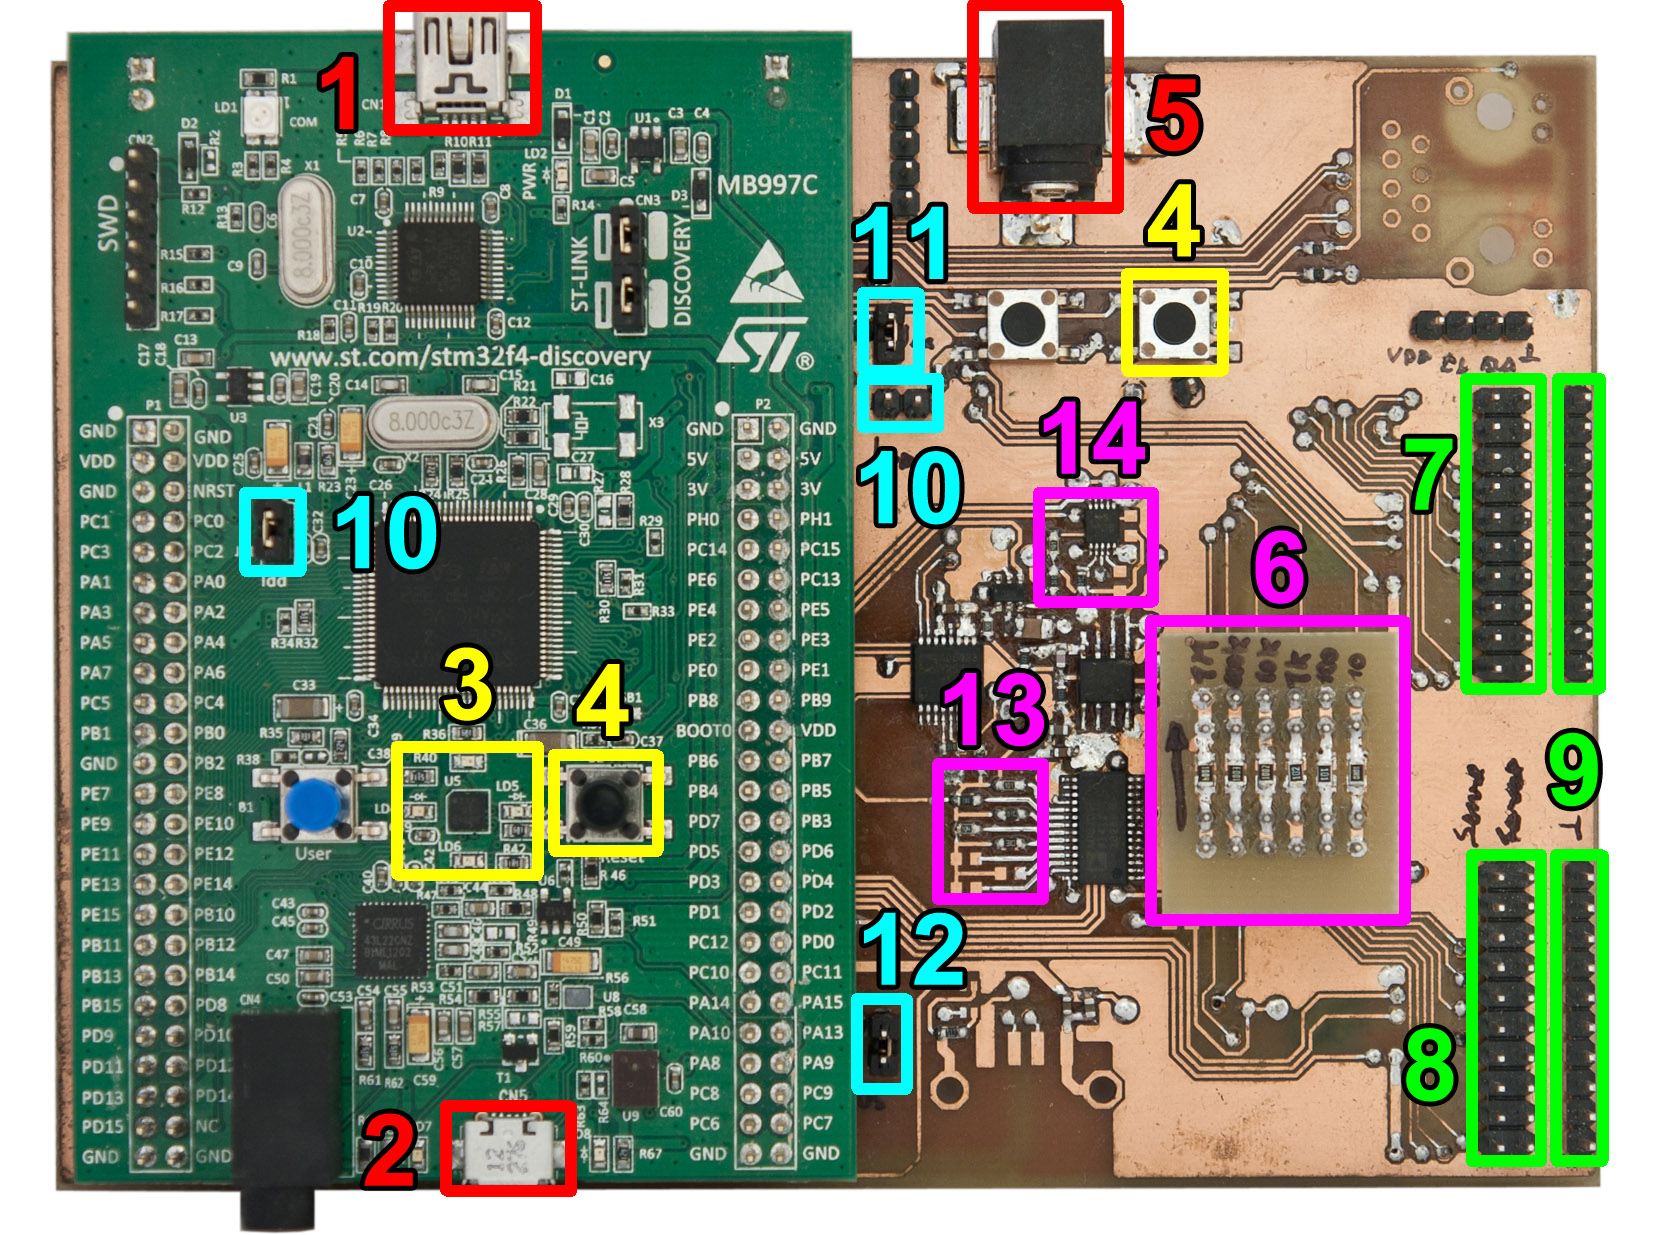
\includegraphics[width=\textwidth]{bilder/device_connections.jpg}
  \caption[Interface on the assembled impedance spectrometer]{
    Interface on the assembled impedance spectrometer:
    \begin{enumerate*}[label=\textbf{\arabic*}, itemjoin={{ -- }}]
      \item \label{itm:usb_prog}  USB programming and power connector
      \item \label{itm:usb_dev}   device USB connector
      \item \label{itm:leds}      status LEDs
      \item \label{itm:btn_rst}   reset button
      \item \label{itm:dc_jack}   DC power jack
      \item \label{itm:r_cal}     board with calibration resistors
      \item \label{itm:meas_out}  measurement output connections, sense (left) and force (right)
      \item \label{itm:meas_in}   measurement input connections (same as output)
      \item \label{itm:meas_gnd}  ground connections
      \item \label{itm:jump_idd}  $ I_\text{DD} $ measurement jumper
      \item \label{itm:jump_icc}  $ I_\text{CC} $ measurement jumper
      \item \label{itm:jump_vbus} $ V_\text{BUS} $ jumper
      \item \label{itm:r_fb}      feedback resistors
      \item \label{itm:r_att}     attenuation resistors
    \end{enumerate*} }
  \label{fig:device_connections}
\end{figure}

The USB programming connector \ref{itm:usb_prog} is used to program and debug the device, it can also be used to power
the device from a standard phone charger or similar supply with a Mini-B USB plug.
The device USB connector \ref{itm:usb_dev} is used to connect the device to a PC and control it.
The DC jack \ref{itm:dc_jack} is a standard \unit{2.5}{\milli\meter} jack (center positive) and can be used to
power the device with a \unit{5}{\volt} DC supply.

When using the device with an external power supply, or powered from the programming connector \ref{itm:usb_prog},
the $ V_\text{BUS} $ jumper \ref{itm:jump_vbus} may be disconnected to prevent the board from drawing power from the
device connector \ref{itm:usb_dev}.

The jumpers \ref{itm:jump_idd} and \ref{itm:jump_icc} can be used to measure the current consumption of the
microcontroller and all the other parts, respectively (note that there are two jumpers for $ I_\text{DD} $,
one on the STM32F4 Discovery board and one on the board, and care should be taken to use only one).

There are four status LEDs \ref{itm:leds}, three of which are used at this time:
\begin{itemize}
	\item \textbf{\color{blue} blue} will blink when the device is powered on, indicating that the firmware
    hasn't locked up,
  \item \textbf{\color{OliveGreen} green} will light up while a measurement is in progress, allowing the user
    to see when it has finished,
  \item \textbf{\color{red} red} will be turned on in case of an error in the firmware, this means the device
    should be reset using the reset button \ref{itm:btn_rst} and the steps leading up to the error should be
    documented, allowing the programmer to fix it.
\end{itemize}

\subsection{First Steps}

Before powering up the device for the first time, the following things should be checked:
\begin{itemize}
	\item the STM32F4 discovery board is properly connected,
  \item a board with calibration resistors is connected to the calibration pins \ref{itm:r_cal},
  \item the necessary feedback and attenuation resistors \ref{itm:r_fb} and \ref{itm:r_att} are soldered on,
  \item the current measurement jumpers \ref{itm:jump_idd} and \ref{itm:jump_icc} are connected
    (or a current meter of course),
  \item the $ V_\text{BUS} $ jumper \ref{itm:jump_vbus} is connected when no external power supply is used.
\end{itemize}

After connecting the device to a PC, any application that can access a serial port can be used to communicate with it.
Settings such as baud rate or parity don't matter.
When not using the MATLAB functions (see \autoref{sec:matlab}), the device is configured via a simple virtual console
interface using human readable commands. Using the \command{help} command, a list of possible commands and their
explanations can be displayed.

The following steps assume the device is fitted with an EEPROM for configuration storage.
The first thing to do after assembling the device is to configure the fitted calibration and feedback resistors, as well
as possible attenuations and the coupling capacitor time constant using the \command{setup} command:
\begin{itemize}
	\item enter possible output voltage attenuations in the order they are selected with the attenuation multiplexer:
    \command{setup attenuation <values>...}
  \item enter feedback resistor values in the order they are connected to the feedback multiplexer in ohms:
    \command{setup feedback <values>...}
  \item enter calibration resistor values in the order they are soldered on the little resistor board (right to left):
    \command{setup calibration <values>...}
  \item enter the coupling capacitor time constant in ms (calculated by $ C_\text{coupl} \cdot \unit{1.1}{\kilo\ohm} $):
    \command{setup coupl <milliseconds>}
\end{itemize}
Typing \command{help setup} shows other options for the \command{setup} command, however none of them are currently
used since the respective peripherals are not yet implemented.


\section{Making Measurements}

After the first steps have been completed, measurements can be performed.
